\label{sec:RESULTS}

\subsection{THE MACH ZEHNDER INTERFEROMETER}
The team began by visualizing the layout of the interferometer given the limited space dictated by the dimension of the optical table. Later, the team aligned the LASER along an axis on the table, filtered the light with a spatial filter and collimated the beam with a optical lens. This is done by placing the lens at its focal point along position 1 in figure \ref{fig:Setup_MZ}. 

We proceeded to build the optical layout for the Mach Zehnder interferometer until we obtained interference patterns. The setup of the Mach-Zehnder interferometer is presented in figure \ref{fig:Setup_MZ}. One of the clear advantages of this interferometer is that both interfering beams travel independent paths. This means it is possible to affect one beam of light by changing one of its characteristics and directly study how interference behaves. 

\begin{figure}[H]
    \centering
    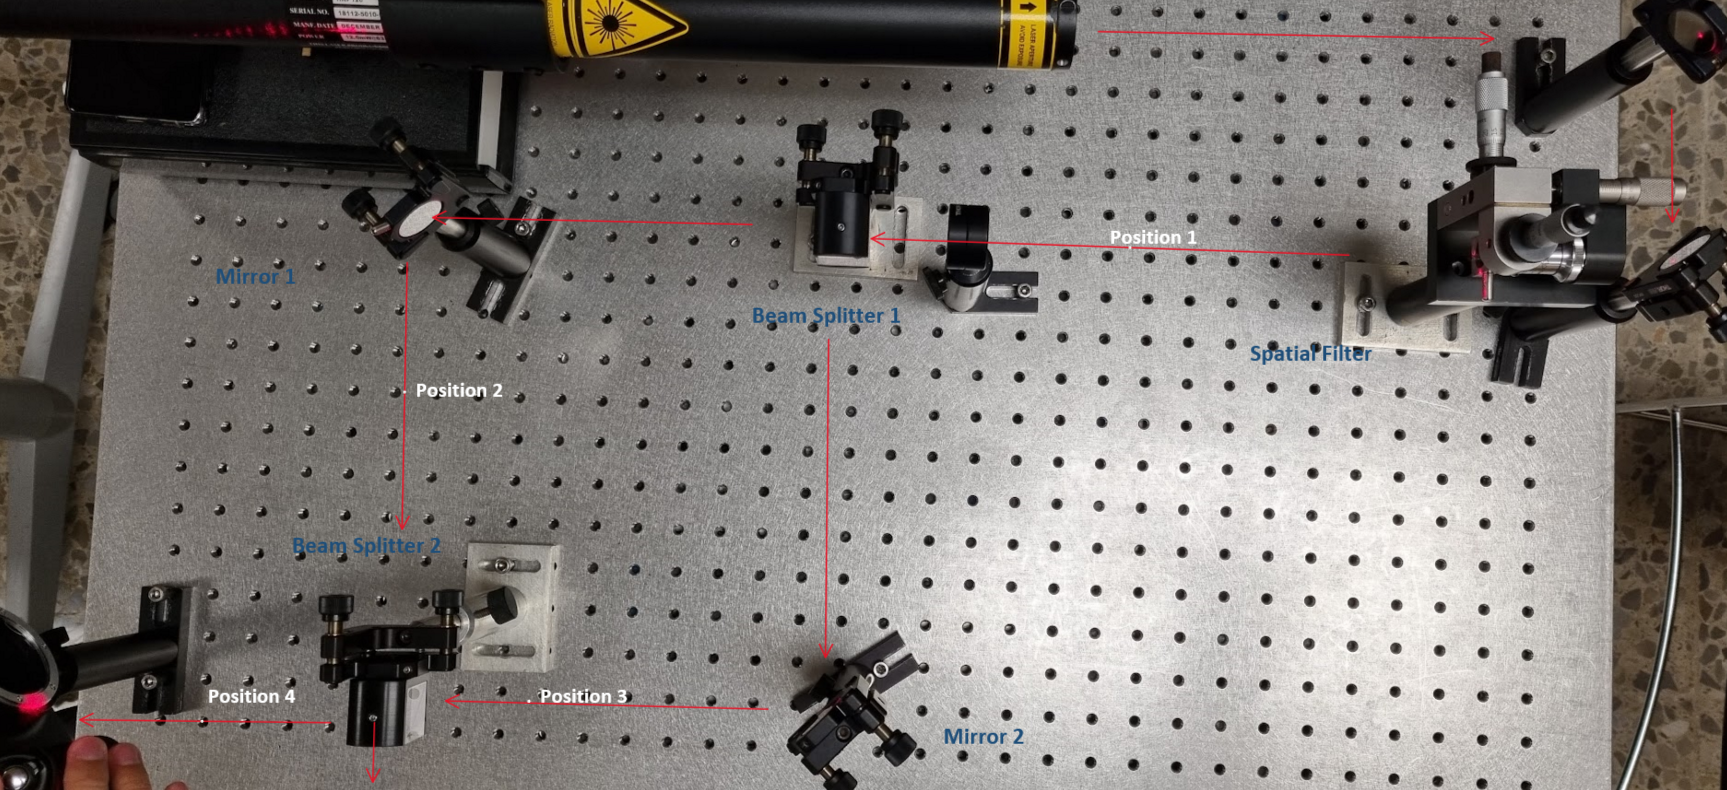
\includegraphics[scale=0.20]{Figures/Figures_I/Mach_Zehnder_ExperimentalSetup.png}
    \label{fig:Setup_MZ}
    \caption{Mach Zehnder experimental layout.}
\end{figure}

While operating the interferometer the team noted that when the beam splitter is slightly tampered, the fringes wiggle maintaining its spatial orientation like shown in figure \ref{fig:Tampered_MZ}. This is because the two interfering beams get affected by the tampering in different ways introducing a very strange phase difference. This is one of the big disadvantages of Mach Zehnder: it is very sensible to environmental noise.

\begin{figure} [H]
    \includegraphics[width=.20 \textwidth]{Figures/Figures_I/DSC_0001.JPG}\hfill
    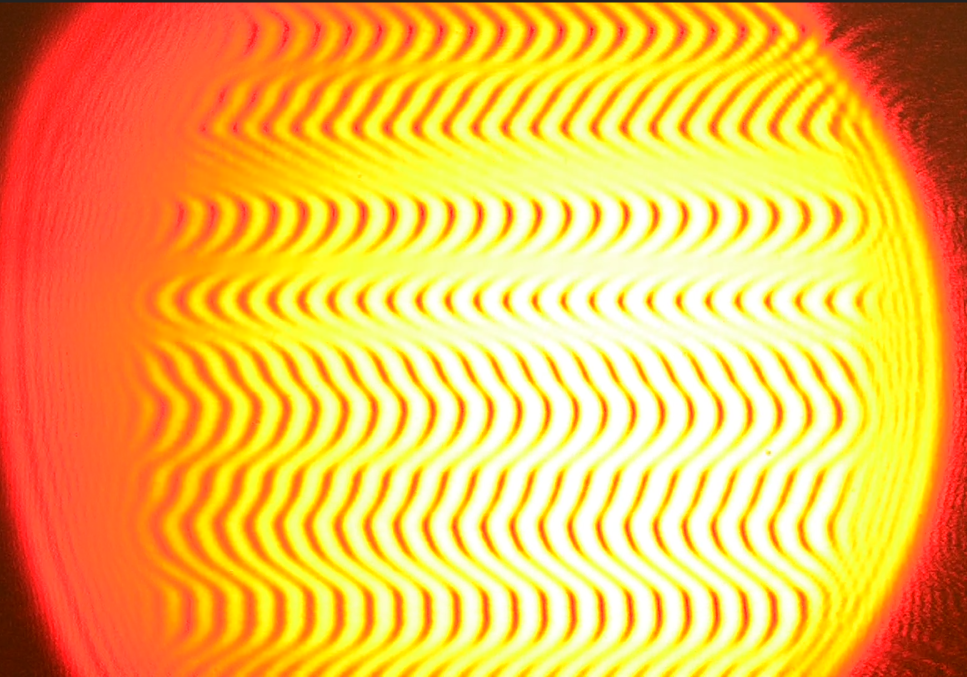
\includegraphics[width=.20\textwidth]{Figures/Figures_I/Tampered_MZ.png}\hfill
    \caption{Reference vs Tampered interference patterns observed by the camera.}
    \label{fig:Tampered_MZ}
\end{figure}

Later we proceeded to test the interference under different conditions. First, we introduced a flame to one of the paths. When we apply a flame to one of the interferometers arms, the fringes seem to amplify ,deform and loose contrast. This can be explained because light from a flame is not polarized. Hence most of the light does not interfere with the beams and we observe low contrast because we introduced some background light. Deformation can be explained because the density of air is compromised by the flame and this introduces a change in the optical path of one of the beams. This changes the phase of the resulting wave and becomes this visible effect illustrated in figure \ref{fig:FlameMZ}.  

\begin{figure}[H]
    \centering
    \includegraphics[scale=0.09]{Figures/Figures_I/Flame_MZ.JPG}
    \label{fig:FlameMZ}
    \caption{One of the arms is introduced a flame.}
\end{figure}

Minor alterations on the mirrors drastically affect the system. By moving the orientations \footnote{In the order of millimeters} of the mirrors in one of the arms we can introduce a variation in the angles between the vectors of propagation $\vec{k_1} $ and $\vec{k_2}$ corresponding to the two interfering beams. This leads to more or less fringes -and their orientation- in the interference patterns. 

\begin{figure} [H]
    \includegraphics[width=.20 \textwidth]{Figures/Figures_I/Mirror_Movment1.JPG}\hfill
    \includegraphics[width=.20\textwidth]{Figures/Figures_I/Mirror_Movment2.JPG}\hfill
    \caption{Interference patterns by phase difference observed by the camera.}
    \label{fig:kvectors}
\end{figure}

Another important observation is when the team introduced a intensity filter (0.5 ND) along one of the Mach Zehnder´s arms (Position 2). As shown in figure \ref{fig:filters}, the contrast of the fringes decreases notably.  This is due because the filter absorbs intensity that would otherwise be interfering with the other beam. Therefore, taking as a reference figure \ref{fig:filters} A; we can observe a difference in contrast. With the filter configuration, the fringes show a lower contrast. 

\begin{figure} [H]
    \includegraphics[width=.20 \textwidth]{Figures/Figures_I/MZ_Filter0.3.JPG}\hfill
    \includegraphics[width=.20\textwidth]{Figures/Figures_I/MZ_NoFilter.JPG}\hfill
    \caption{Filtered vs Non Filtered interference patterns observed by the camera.}
    \label{fig:filters}
\end{figure}

\subsection{POLARIZATION EFFECTS}

In section \ref{sec:TEO_FRAMEWORK} we discussed that a shared state of polarization is needed in order to interference to emerge. To test this statement empirically, we introduced in position 3 (Figure \ref{fig:Setup_MZ}) a half wavelength $\lambda /2$ retarder at a $45 ^o $ degree angle from its fast axis which in turn matches the orientation of the polarized state of the beam. This inverts the polarization on the beam by $90 ^o $ degree. At this point (Figure \ref{fig:polMZ} A), the two beams do not form interference because the polarization states are perpendicular to each other. Then the team adjusted the angle of the $\lambda /2$ retarder to $0 ^o $ -I.e not affecting the initial polarization state - we observe the interference pattern once again (Figure \ref{fig:polMZ} B). The team later proceeds to introduce the two perpendicular polarization states until the interference fringes disappear. To recover the interference patterns once again, we first mounted a linear polarizer in position 4. By aligning the polarizer to a $45 ^o $ degree angle from the vertical state of the LASER we observed the fringes once again (Figure \ref{fig:polMZ} C)! This is because the interfering vertical and horizontal states can be thought of a superposition of a diagonal and anti diagonal states. In linear algebra this is known as a chance of basis. Thus, the diagonal polarizer in position 4 allows both beams to interfere in its diagonal polarization state and the observation leads to fringes. 

\begin{figure} [H]
    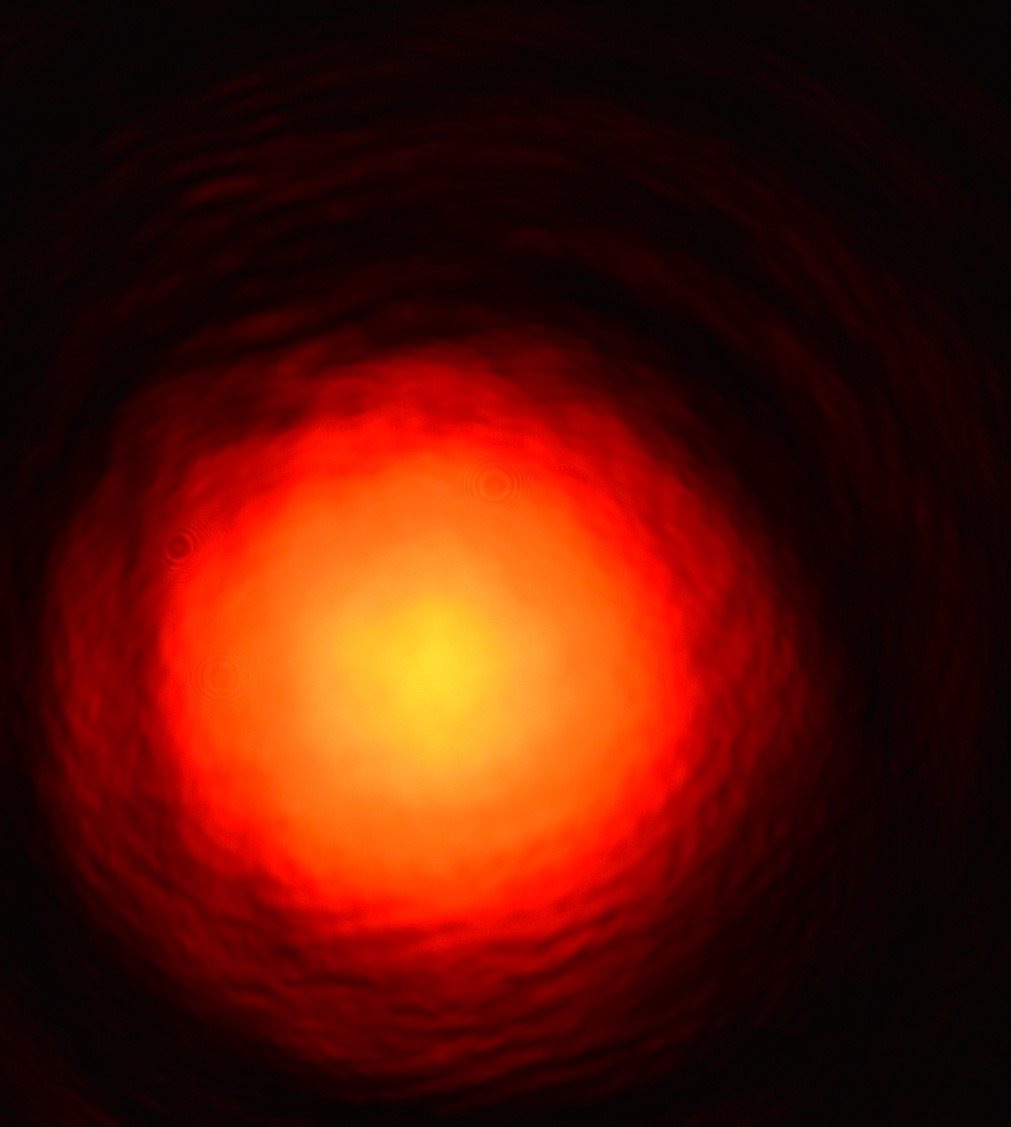
\includegraphics[width=.14 \textwidth]{Figures/Figures_I/MZ_Fringes (3).JPG}\hfill
    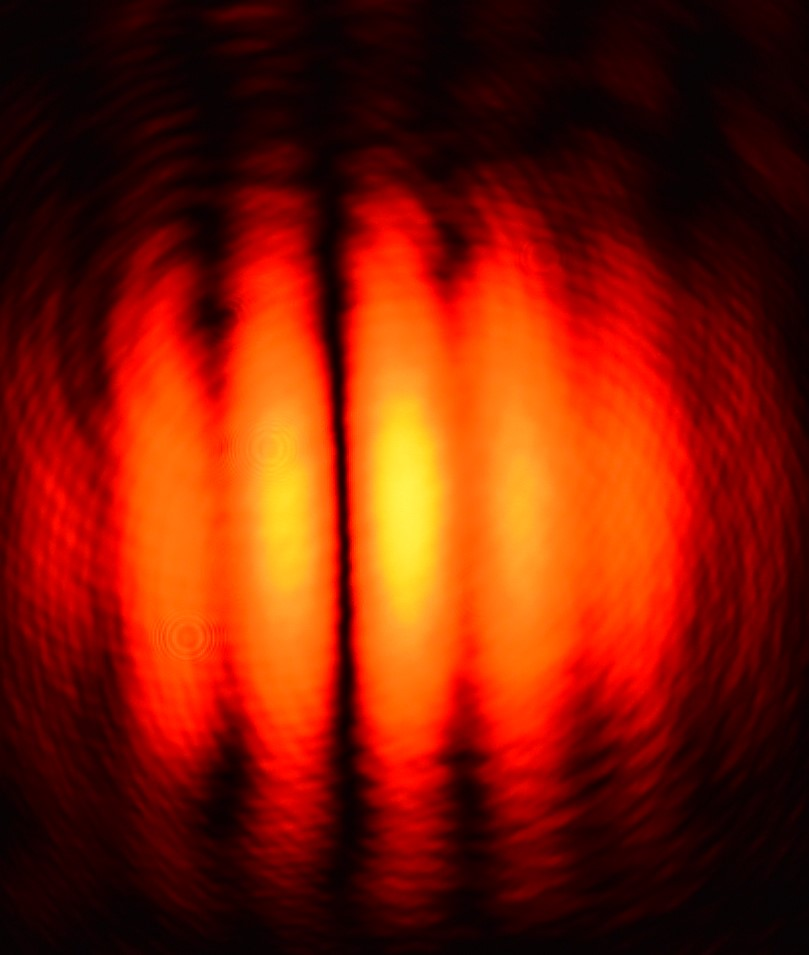
\includegraphics[width=.13\textwidth]{Figures/Figures_I/MZ_Fringes (4).JPG}\hfill
    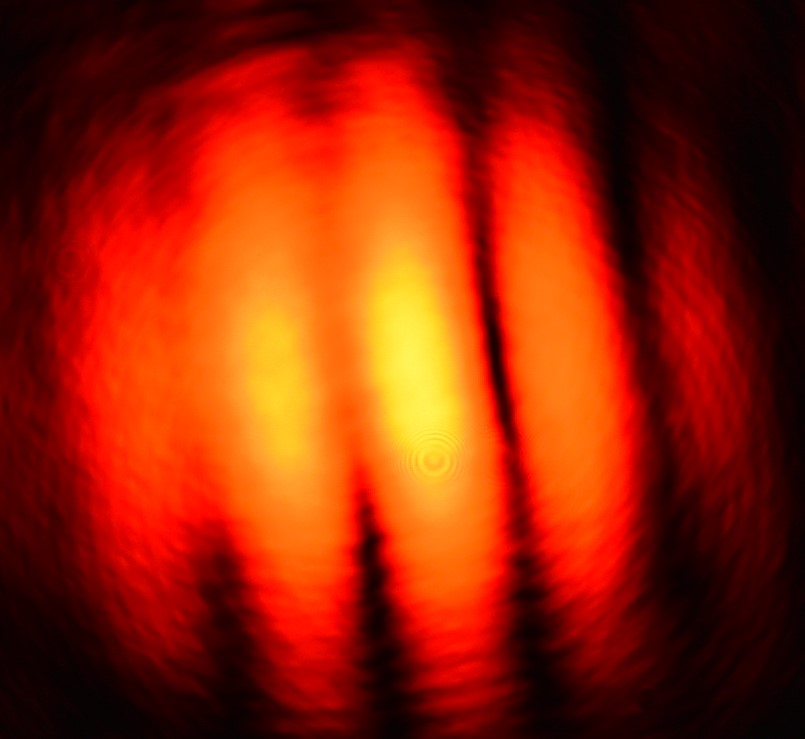
\includegraphics[width=.17\textwidth]{Figures/Figures_I/MZ_Fringes (5).JPG}\hfill
    \caption{A) No interference because of perpendicular polarization states. B) Interference because 2 parallel polarization states. C) Interference because perpendicular states interfere in a diagonal polarized orientation. }
    \label{fig:polMZ}
\end{figure}


\subsection{PHASE RETARDATION BY $\Delta \Lambda$}
In the previous subsection the team found that introducing a different air density -due to the presence of a flame- in one of the interferometers arms leads to different interference patterns. This is because a difference in the optical path $\Delta \Lambda$ is introduced and the beams interfere with each other at different phases. To test this phenomena in a more controlled matter, the team proceeded to introduce a glass plate in position 2 (Figure \ref{fig:Setup_MZ}). This made one of the beams refract and thus introducing a $\Delta \Lambda$. Figure \ref{fig:GlassSetup} is a picture of the visible interference affected by the glass (white borders) and the unaffected by the glass on the bottom of the picture.
\begin{figure}[H]
    \centering
    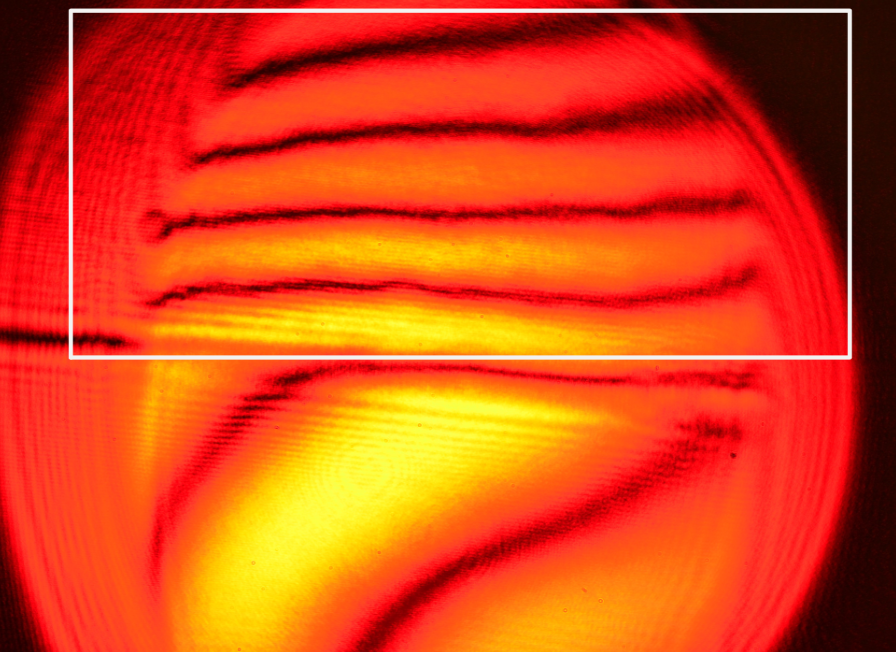
\includegraphics[scale=0.20]{Figures/Figures_I/GlassOneArm_MZ.png}
    \label{fig:GlassSetup}
    \caption{Glass applied to half of a beam in position 2 at an angle.}
\end{figure}
Two facts are very clear from figure \ref{fig:GlassSetup}: 1) the refraction angle caused by the glass shifts the vector of propagation in one of the beams and thus generates different number of fringes and 2) different orientations. 

\subsection{INTERFERING WAVE FRONTS}
Finally the team set up a configuration to study the interference of two different types of wave-fronts: plane waves and spherical waves. To achieve this, we introduced a lens on position 3 (Figure \ref{fig:Setup_MZ}). This focuses the incident plane (or collimated) wavefront generating a spherical wavefront. After this two wave-fronts interfere the following interference pattern emerges \cite{fig:Wavefronts}: 
\begin{figure}[H]
    \centering
    \includegraphics[scale=0.10]{Figures/Figures_I/Wavefronts_MZ.JPG}
    \label{fig:Wavefronts}
    \caption{Plane and spherical interfering wave-fronts.}
\end{figure}
The results are not good quality because of poor collimation techniques. However, during the experiment we observed that an array of concentric circles begins to form when these two wave-fronts interfere. 

\subsection{ALTERNATIVE INTERFEROMETERS BY PHASE DIVISION} 

Other configurations involving beam splitters include the Michelson and Sagnac configurations (Figure \ref{fig:MS}. They have other strong characteristics that can allow physicists to measure different characteristics of the interference phenomena. 

\begin{figure}[H]
    \centering
    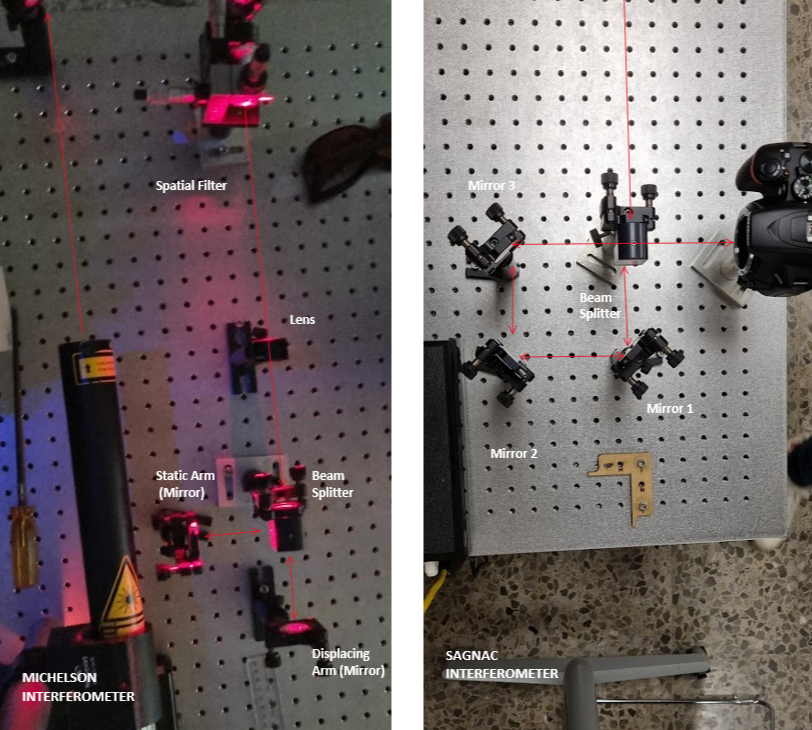
\includegraphics[scale=0.33]{Figures/Figures_I/MichelsonSagnac.png}
    \label{fig:MS}
    \caption{A) Michelson and B) Sagnac interferometer.}
\end{figure}

We will use this space to answer what I consider 3 pertinent questions about the phenomena of interference. 
\begin{enumerate}
    \item What happens to the energy when we have destructive interference?
    
    \item What is the coherence of our LASER BEAM listed in section \ref{sec:mat}? 
    %\item What are the conditions to generate a wavefront with multiple polarization distributions? 
\end{enumerate}

The Sagnac interferometer was used by the team to measure the distribution of energy in the beam. The team built the configuration illustrated in figure \ref{fig:MS}, later a series of pictures where taken in order to obtain different fringe numbers and registering as matrix digital measurements. The integral of this transversal measurement can be related to the energy as displayed in (Figure \ref{fig:SagResult}). Resolving question 1): In regions of destructive interference, energy is in a different configuration state but still conserved due to compensation in regions inside the constructive case.
\begin{figure}[H]
    \centering
    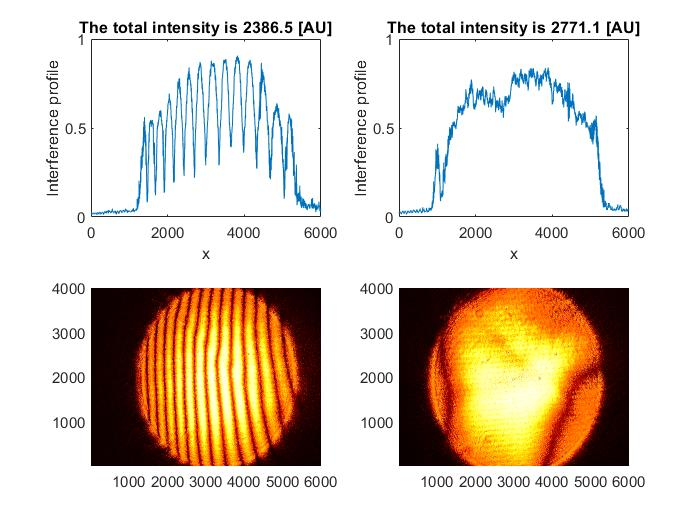
\includegraphics[scale=0.25]{Figures/Figures_I/SagnacResult_EnergyConservation.jpg}
    \label{fig:SagResult}
    \caption{Energy conservation readings match up to value of $92\%$ of energy conservation. }
\end{figure}

Michelson's interferometer its optimal for experiments involving displacements in mirror. Thus, this configuration will allow the team to perform measurements of the coherence of the LASER. The team began re calibrating the interferometer. Later, we proceeded to move the mirror such that $l_0 -> 0$ and stop when we no longer observe where the interference (Figure \ref{fig:MichRes}). The measured value was $x_{I0} =0.00 cm $. Later we varied $l_0 -> \inf$ because the nature of the LASER is not purely monochromatic, the coherence of the beam will hold for a finite range of distance values . We observed a distance where the fringes are no longer distinguishable. That distance is recorded as $x_{IF} =102.00 cm $. E.i the coherence distance ($\chi$) is 
\begin{equation} 
\chi = x_{IF} - x_{I0} = 102 cm, 
\end{equation} 
is related to the temporal coherence discussed in section \ref{sec:TEO_FRAMEWORK} by introducing the velocity (c)
\begin{equation} 
\tau = \chi / c [s]. 
\end{equation} 
Therefore after $\tau$ seconds, the LASER light decoheres. 
\begin{figure} [H]
    \includegraphics[width=.20 \textwidth]{Figures/Figures_I/DSC_0323.JPG}\hfill
    \includegraphics[width=.20\textwidth]{Figures/Figures_I/DSC_0321.JPG}\hfill
    \caption{$x_{IF}$ and $x_{I0}$ experimental results (respectively). }
    \label{fig:MichRes}
\end{figure}



%For the final part of this practice the team build Sagnac's Interferometer (Figure\ref{fig:MS}) with a polarized beam splitter \footnote{Where the reflected beam is horizontal and the transmitted beam is vertical.}. We measured stokes parameters to obtain wave fronts with different polarization distributions. We start by rotating the linear polarizer in position 2 \ref{fig:MS} to measure stokes parameter of the two incident opposite circular polarization states this has the effect of shifting the fringe pattern a multiple $pi/4$. Thus, when calculating stokes \footnote{A series of parameters that allow to describe the polarization state of an optical system} for $ S_3 $ we will have a matrix whose values range from -1 to 1. This means some regions have elliptical R polarization (positive $S_3$) and other regions have the opposite polarization (negative $S_3$values). Figure \ref{} illustrates this wavefront distribution of a measure result. 

